\section{Methodische Vorgehensweise}
\subsection{Datenerhebung}
Für die Gegenüberstellung der Technologietrends in der akademischen Forschung und praktizierenden Wirtschaft werden, wie bereits in Abschnitt \ref{sec:method} erwähnt, zwei Arten von Quellen herangezogen.

\subsubsection{Gartner Hype Cycle for Emerging Technologies}\label{sec:ghcet}
Der \glqq Gartner Hype Cycle for Emerging Technologies\grqq~repräsentiert als markt\-führendes Beratungsunternehmen für Technologieprognosen den Part der praktizierenden Wirtschaft. Dabei dienen die Technologien in der Phase \glqq Peak of Inflated Expectations\grqq~in vorliegender Reihenfolge als Datenbasis für die Analyse, da sie den Höhepunkt der Trendwahrnehmung darstellen.

Eine komplette Ausgabe inklusive der Erläuterungen einzelner Phasen sowie der aufgeführten Technologien ist kostenpflichtig über den Webauftritt des Unternehmens: \url{https://www.gartner.com} erhältlich. Für die vorliegende Untersuchung ist sie jedoch nicht erforderlich, da die notwendigen Informationen in Unterpfaden der Webseite frei erhältlich sind.

Die graphische Darstellung des \glqq Hype Cycle for Emerging Technologies \grqq~wird jährlich in Form eines Nachrichtenartikels frei veröffentlicht.\footnote{\citeNP<Vgl.>[o.S.]{ghcet2016}}
Die genaue Aufteilung der Technologien in die fünf bekannten Phasen ist wiederum der Webseite, wo der Artikel gekauft und heruntergeladen werden kann, aus dem dort aufgeführten Inhaltsverzeichnis zu entnehmen.\footnote{\citeNP<Vgl.>[o.S.]{ghc2016}}

Für die optimale Ausrichtung der Analyse an die Leitfragen ist es sinnvoll, eine relativ aktuelle Ausgabe des \glqq Hype Cycle\grqq~zu verwenden, nicht jedoch die neuste. Denn für die Leitfrage L3 wird mindestens eine neuere Ausgabe als die analysierte benötigt. Bei zu alten Publikationen besteht wiederum die Gefahr, dass durch gegenseitige Einflussnahme eine Angleichung bspw. der Begrifflichkeiten die Ergebnisse verfälschen könnte.

Die aktuellste Ausgabe des \glqq Gartner Hype Cycle for Emerging Technologies\grqq~ ist im Juli 2017 erschienen.\footnote{\citeNP<Vgl.>[o.S.]{ghc2017}} Deshalb fällt die Wahl auf die unmittelbar vorausgegangene Veröffentlichung aus dem Jahre 2016. In der Phase \glqq Peak of Inflated Expecta\-tions\grqq~sind folgende Technologien aufgeführt:\footnote{\citeNP<Vgl.>[o.S.]{ghc2016}}

\begin{itemize}
	\item Gesture Control Devices
	\item Micro Data Centers
	\item Smart Robots
	\item Blockchain
	\item Connected Home
	\item Cognitive Expert Advisors
	\item Machine Learning
	\item Software-Defined Security
	\item Autonomous Vehicles
	\item Nanotube Electronics
	\item Software-Defined Anything (SDx)
\end{itemize}

In Abbildung \ref{fig:ghc2016} ist der dazugehörige Graph zu sehen, dem zusätzlich die Erwartungen an die Technologie in Abhängigkeit zum Reifegrad sowie die voraussichtliche Dauer bis zur Erreichung des \glqq Plateau of Productivity\grqq~entnommen werden können.

\begin{figure}[ht]
	\centering
	\caption{Gartner Hype Cycle for Emerging Technologies, 2016}
	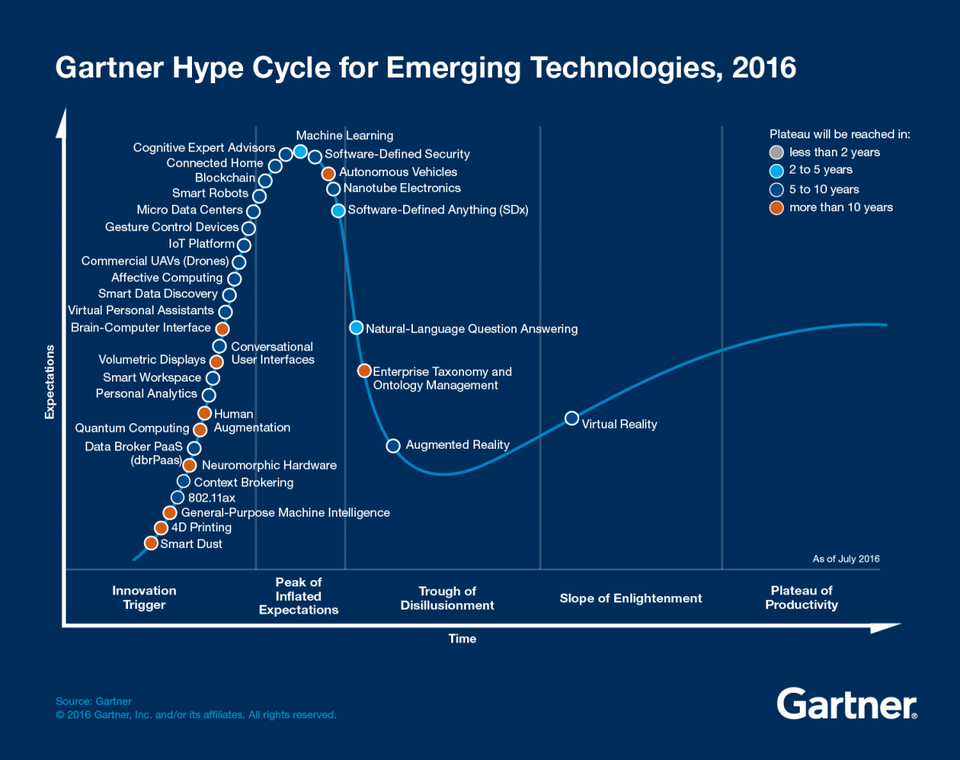
\includegraphics[width=0.9\linewidth]{img/Hype_Cycle_2016.jpg}
	\caption*{\protect\citeNP<Quelle:>[o.S.]{ghcet2016}}
	\label{fig:ghc2016}
\end{figure}

Demnach waren beispielsweise die Erwartungen und somit die Trendwahrnehmung für die Technologie \glqq Machine Learning\grqq~im Jahre 2016 am höchsten. Die Technologien links davon hatten eine geringere Reife, die rechts davon eine höhere. Insgesamt handelt es sich bei den Technologien allesamt um Trends des Jahres 2016 in der praktizierenden Wirtschaft.

Um den Trendverlauf der ausgewählten Technologien zu bestimmen, müssen weitere \glqq Hype Cyles\grqq~betrachtet werden. Das erstmalige Erscheinen in einer Publikation liefert einen Hinweis darauf, wann eine Technologie die Aufmerksamkeit der relevanten Gruppe von praktizierenden Wirtschaftlern erlangt hat. Die Verteilung der Vorkommnisse und Abwesenheiten der Technologien in den jeweiligen Ausgaben ermöglicht Rückschlüsse über den Zeitraum und Verlauf der Trendwahrnehmung.

Zur Ermittlung des erstmaligen Erscheinens werden solange vergangene \glqq Hype Cycles\grqq~betrachtet, bis die jeweils gesuchte Technologie in einer vorhergehenden Ausgabe fehlt. Für die meisten Technologien ist damit das Jahr der ersten Ausgabe ermittelt. Ist die Prognose der Dauer bis zum Erreichen des \glqq Plateaus\grqq~ mit größer als fünf Jahren angegeben, sind weitere Vorgänger zu betrachten, da eine Technologie in der Zeit vorübergehend unter die Trendschwelle fallen kann.

Für die Ermittlung des Trendverlaufs wird zusätzlich die aktuelle Ausgabe hinzugenommen.

Dabei sind folgende Parameter für die Auswertung festzuhalten:

\begin{enumerate}
	\item Name der Technologie
	\item Jahr aller Erscheinungen mit Zuordnung zur jeweiligen Phase
	\item Position innerhalb der entsprechenden Phase
\end{enumerate}

\subsubsection{Literaturdatenbanken}\label{sec:lit_data}
Demgegenüber wird die Datenbasis der akademischen Forschung aus Abfragen in relevanten Literaturdatenbanken erhoben. Aufgrund ihrer hohen Abdeckung wissenschaftlich, technologischer Publikationen werden folgende Datenbanken durchsucht:
\begin{description}
	\item [WoS:] Web of Science Core Collection - \url{http://apps.webofknowledge.com}
	\item [IEEE:] IEEE Xplore Digital Library - \url{https://ieeexplore.ieee.org}
	\item [ACM:] The ACM Guide to Computing Literature - \url{https://dl.acm.org}
\end{description}

Diese enthalten neben den in Abschnitt \ref{sec:acad_pub} genannten Fachzeitschriften und Tagungsbänden weitere Formen von Veröffentlichungen, wie beispielsweise Bücher oder Standards. Daher ist die Suche ausschließlich darauf einzugrenzen, wobei die Ergebnisse nach Veröffentlichungsform getrennt voneinander gehalten werden, da dies genauere Rückschlüsse über den tatsächliche Verlauf ermöglicht.

Alle Suchmaschinen sind im erweiterten Suchmodus mit vergleichbarer Funktionalität zur Vergabe von Suchkriterien ausgestattet. Diese sind gezielt einzusetzen, damit das Suchergebnis einerseits möglichst vollständig ist und andererseits keine \glqq False Positives\grqq~liefert. Deshalb beschränkt sich die Suche der Technologien auf die Metadaten Titel, Stichwörter und Abstract einer Publikation.

Der erweiterte Suchmodus bietet in allen Suchmaschinen die Möglichkeit, Suchanfragen mittels Kommandoanweisungen einzugeben. Die Operatoren zur Verknüpfung von Suchbegriffen sind nahezu identisch, wobei die Syntax einer Suchanweisung teilweise unterschiedlich ist. Somit sind die Querys untereinander nicht wahllos austauschbar. Bei IEEE und ACM können einige Suchkriterien wie beispielsweise die Veröffentlichungsform nicht über das Kommando eingegeben werden, sondern müssen durch entsprechende Auswahl mithilfe von Bedienelementen in der Web\-oberfläche erfolgen.

Im ersten Schritt werden die Technologien aus Abschnitt \ref{sec:ghcet} unverändert in die Suchmaschine eingegeben, um einen ersten Eindruck der Datenlage im Hinblick auf potentielle Unterschiede bei den Begrifflichkeiten zu erhalten. Mit den oben genannten Eingrenzungen ergibt das für den Begriff \glqq Machine Learning\grqq~in Fachzeitschriften folgende Suchalgorithmen je Suchmaschine:

\begin{description}
	\item [WoS:] \begin{verbatim}
	(TS=("machine learning")) AND DOCUMENT TYPES: (Article)
	\end{verbatim}

	\item [IEEE:] \begin{verbatim}
	("machine learning")
	\end{verbatim}
	Zusätzliche Filtereinstellungen:
	\begin{itemize}
		\item Search Context: Metadata only
		\item Content Types: Journals \& Magazines
	\end{itemize}

	\item [ACM:] \begin{verbatim}
	acmdlTitle:(+"machine learning") OR
	recordAbstract:(+"machine learning") OR
	keywords.author.keyword:(+"machine learning")
	\end{verbatim}
	Zusätzliche Filtereinstellung:
	\begin{itemize}
		\item Refine by Publications / All Publications / Periodical
	\end{itemize}
\end{description}

Für die Ermittlung der idealen Suchalgorithmen ist es wichtig, die im \glqq Hype Cycle\grqq~vorkommenden Technologiebegriffe genau zu verstehen. Dies gilt insbesondere, wenn diese mit der wissenschaftlichen Benennung nicht exakt übereinstimmen. Deshalb werden die Technologien zunächst in Gartners IT-Glossar\footnote{\url{https://www.gartner.com/it-glossary/}} verifiziert.

Im nächsten Schritt gilt es, alternative Bezeichnungen der Technologiebegriffe aus dem \glqq Hype Cycle\grqq~herauszufinden, um eine möglichst vollständige Abdeckung von Publikationen zu den entsprechenden Technologien zu erhalten. Dazu werden die Stichwörter der einzelnen Suchergebnisse stichprobenartig nach Synonymen durchsucht, welche anschließend adjunktiv mit der ursprünglichen Suche verknüpft werden.

Andersherum sind Begriffe auszuschließen, die für eine höhere Evolutionsstufe der ursprünglichen Technologie stehen, diese jedoch signifikant erweitern, so dass ein neuer Begriff einen neuen Kontext rechtfertigt. Ein Beispiel dafür sind die Technologien \glqq Machine Learning\grqq~und \glqq Deep Learning\grqq, welche jeweils ihre eigene Daseinsberechtigung haben und daher in der aktuellen Ausgabe des \glqq Hype Cycle for Emerging Technologies 2017\grqq~im \glqq Peak of Inflated Expectations\grqq~nebeneinander stehen.\footnote{\citeNP<Vgl.>[S.~45.]{ghc2017}} Da es sich bei \glqq Deep Learning\grqq~um die neuere Technologie handelt, wird sie mit dem exkludierenden Operator \glqq NOT\grqq~jeweils herausgenommen.

Für die Auswertung wird die Verteilung der Publikationen pro Jahr und Filter benötigt. Dazu werden die entsprechenden Exportfunktionen der jeweiligen Suchmaschinen eingesetzt. Im WoS ist ein Export der Verteilung von Publikationen pro Jahr von maximal \numprint{200000} Datensätzen mit einer einzigen Anweisung im TSV-Format (Tabulator-Seperated Values) möglich. Die anderen beiden Suchmaschinen erlauben lediglich einen Export von maximal \numprint{2000} Datensätzen der Metadaten im CSV-Format (Comma-Seperated Values). Das bedeutet, dass für Suchergebnisse mit mehr als \numprint{2000} Ergebnissen mehrere Exportanweisungen durchgeführt werden müssen.

\subsection{Operationalisierung der Daten}
Im nächsten Schritt werden die gewonnenen Daten strukturiert, um die Gegenüberstellung der Technologietrends in Wirtschaft und Wissenschaft im Hinblick auf die Beantwortung der Leitfragen zu ermöglichen.

\subsubsection{Verteilung der Technologietrends in der praktizierenden Wirtschaft}
Nachdem die zeitliche Verteilung der Technologien aus Abschnitt \ref{sec:ghcet} ermittelt ist, wird eine Übersicht darüber inklusive weiterer relevanter Daten erstellt. Aus Gründen der Vergleichbarkeit mit der Verteilung der wissenschaftlichen Publikationen eignet sich dazu eine Tabellenform, in der die Technologien in ihrer ursprünglichen Reihenfolge als Zeilenüberschriften und die Veröffentlichungsjahre als Spaltenüberschriften dienen, wie in Tabelle~\ref{tab:dist_ghc} zu sehen ist. Die Technologien werden dabei durch ihre Akronyme abgekürzt, da sie in vorliegendem Fall eindeutig sind und die Tabelle dadurch übersichtlicher wird.

Leere Zellen bedeuten, dass die Technologie im entsprechenden Veröffentlichungsjahr nicht vorkommt. Anderenfalls setzt sich der Eintrag prinzipiell aus zwei Teilen zusammen. Im ersten Teil wird das Kürzel der Phase des \glqq Hype Cyles\grqq~aufgeführt, in der die Technologie vorkommt. Für vorliegende Datenbasis werden folgende Kürzel benutzt:

\begin{description}
	\item[I:] Innovation Trigger
	\item[P:] Peak of Inflated Expectations
	\item[T:] Trough of Disillusionment
\end{description}

Die anderen beiden Phasen bleiben unberücksichtigt, da sie die zu untersuchenden Technologien in keiner Ausgabe enthalten. Der zweite Teil gibt die Position der Technologie unter allen anderen der jeweiligen Phase wieder.

Für die Technologie \glqq Machine Learning\grqq~im Jahre 2016 heißt das bspw., dass sie in der Phase \glqq Peak of Inflated Expectations\grqq~erschienen ist, insgesamt elf Technologien in dieser Phase vorkommen und \glqq Machine Learning\grqq~an Position sieben zu finden ist. Zusätzlich wird die Spalte des zugrundeliegenden Jahres mit einem Sternchen (*) gekennzeichnet, falls es sich bei der Technologie um den höchsten Punkt der Kurve handelt.

\begin{table}
	\caption{Verteilung der Technologien des \glqq Gartner Hype Cycle\grqq}
	\centering
	\label{tab:dist_ghc}
\begin{tabularx}{\linewidth}{X|XXXXXXX}
	& 2010 & 2012 & 2013 & 2014 & 2015 & 2016 & 2017 \\
	\hline
	GCD &  &  &  &  &  & P 1/11 &  \\
	\hline
	MDC &  &  &  &  & P 2/10 & P 2/11 &  \\
	\hline
	SR &  &  &  & I 13/17 & I 11/18 & P 3/11 & P 3/13 \\
	\hline
	B &  &  &  &  &  & P 4/11 & P 12/13 \\
	\hline
	CH &  &  &  & I 5/17 & I 13/18 & P 5/11 & P 6/13 \\
	\hline
	CEA &  &  &  &  &  & P 6/11 & T 1/4 \\
	\hline
	ML &  &  &  &  & P 8/10 & P 7/11* & P 8/13 \\
	\hline
	SDS &  &  &  &  & I 18/18 & P 8/11 & T 3/4 \\
	\hline
	AV & I 7/12 & I 7/9 & I 12/14 & P 3/10 & P 5/10* & P 9/11 & P 9/13 \\
	\hline
	NE &  &  &  &  &  & P 10/11 & P 10/13 \\
	\hline
	SDx &  &  &  &  &  & P 11/11 &  \\
\end{tabularx}
\caption*{Quelle: Eigene Darstellung}
\end{table}

\subsubsection{Verteilung der Technologietrends in der wissenschaftlichen Forschung}
Die Übersicht der Verteilung zu vergleichender Technologien wird ebenfalls tabellarisch aufgebaut. Der Vergleichbarkeit halber werden die Zeilen- und Spaltenüberschriften möglichst identisch zur Vergleichsbasis aus Tabelle \ref{tab:dist_ghc} gehalten. Um dabei die Lesbarkeit zu wahren, werden zusätzliche Veröffentlichungsjahre der Vergangenheit an dieser Stelle kumuliert. Da die Zeitspanne der Veröffentlichungsjahre sich teilweise über mehrere Jahrzehnte erstreckt, wäre andernfalls ihre Darstellung in einer Zeile nicht möglich. Für die Analyse werden jedoch die Rohdaten verwendet, die auch im Anhang wiederzufinden sind. Die Zeilenüberschriften bedürfen hingegen keiner Anpassung. Die Tabellenzellen wiederum beinhalten die Anzahl an Publikationen zu einer Technologie in dem entsprechenden Jahr.

Zusätzlich werden die nach dem in Abschnitt \ref{sec:lit_data} beschriebenen Vorgehen ermittelten Suchalgorithmen erfasst, um eine Reproduzierbarkeit der Analyse zu gewährleisten. Zudem wird die Anzahl der Treffer bei einer exakten Suche der Technologie festgehalten.

Da die Ergebnisse der einzelnen Suchmaschinen im ersten Schritt nicht kumuliert werden, entstehen zunächst einmal sechs Tabellen -- eine Tabelle pro Suchmaschine und Veröffentlichungsform.

TODO: Ermittlung der Suchalgorithmen detailliert beschreiben

In Tabelle \ref{tab:dist_wos_art} ist die entsprechende Mengenverteilung der Publikationen in Fachzeitschriften des \glqq Gartner Hype Cycle for Emerging Technologies 2016\grqq~aus Abschnitt \ref{sec:ghcet} zu entnehmen.

\begin{table}
	\caption{Verteilung der Publikationen in Fachzeitschriften im \glqq Web of Science\grqq}
	\centering
	\label{tab:dist_wos_art}
\begin{tabularx}{\linewidth}{X|X|X|X|X|X|X|X|X|X|X}
	& $\leq$~'09 & '10 & '11 & '12 & '13 & '14 & '15 & '16 & '17 & '18 \\
	\hline
	GCD & 8 & - & 1 & 5 & 3 & 11 & 16 & 23 & 16 & 6 \\
	\hline
	MDC & - & - & - & - & - & - & 1 & - & 4 & 3 \\
	\hline
	SR & 609 & 93 & 137 & 160 & 207 & 169 & 250 & 279 & 287 & 164 \\
	\hline
	B & - & - & - & - & - & - & 1 & 28 & 155 & 152 \\
	\hline
	CH & 219 & 48 & 72 & 96 & 120 & 140 & 203 & 244 & 370 & 242 \\
	\hline
	CEA & 2 & - & - & - & - & - & - & - & - & - \\
	\hline
	ML & \numprint{7241} & \numprint{1154} & \numprint{1366} & \numprint{1547} & \numprint{1990} & \numprint{2353} & \numprint{3232} & \numprint{4212} & \numprint{5580} & \numprint{4467} \\
	\hline
	SDS & - & - & - & - & - & 1 & 2 & 3 & 1 & 2 \\
	\hline
	AV & 587 & 80 & 80 & 113 & 91 & 117 & 176 & 237 & 361 & 260 \\
	\hline
	NE & 522 & 106 & 88 & 86 & 61 & 77 & 71 & 94 & 79 & 57 \\
	\hline
	SDx & - & - & - & - & - & - & - & - & - & 1 \\
\end{tabularx}
	\caption*{Quelle: Eigene Darstellung}
\end{table}

\begin{table}
\caption{Verteilung der Publikationen in Tagungsbänden im \glqq Web of Science\grqq}
\centering
\label{tab:dist_wos_proc}
\begin{tabularx}{\linewidth}{X|X|X|X|X|X|X|X|X|X|X}
	& $\leq$~'09 & '10 & '11 & '12 & '13 & '14 & '15 & '16 & '17 & '18 \\
	\hline
	GCD & 3 & - & - & - & - & 1 & - & - & - & 1 \\
	\hline
	MDC & - & - & - & - & - & - & - & - & - & - \\
	\hline
	SR & 202 & 3 & 7 & 4 & 1 & 4 & 10 & 7 & 5 & 8 \\
	\hline
	B & - & - & - & - & - & - & - & - & 5 & 1 \\
	\hline
	CH & 59 & 3 & 3 & 1 & 1 & 2 & 7 & 7 & 16 & 6 \\
	\hline
	CEA & - & - & - & - & - & - & - & - & - & - \\
	\hline
	ML & \numprint{2042} & 64 & 57 & 35 & 61 & 59 & 132 & 164 & 126 & 126 \\
	\hline
	SDS & - & - & - & - & - & 1 & - & - & - & - \\
	\hline
	AV & 103 & 4 & 3 & 5 & 1 & 1 & 4 & 4 & 8 & 9 \\
	\hline
	NE & 65 & 16 & 9 & 1 & 3 & 2 & 4 & 2 & - & - \\
	\hline
	SDx & - & - & - & - & - & - & - & - & - & \\
\end{tabularx}
\caption*{Quelle: Eigene Darstellung}
\end{table}

Die dazugehörigen Suchalgorithmen sind wie folgt:

\begin{description}
	\item[GCD:] \begin{verbatim}(TS=("natural user interface"
	OR "gesture control device"
	OR "gesture control devices")) AND DOCUMENT TYPES: (Article)\end{verbatim}
	\item[MDC:] \begin{verbatim}(TS=("micro data center"
	OR "micro data centers"
	OR "microdata center"
	OR "micro datacenter")) AND DOCUMENT TYPES: (Article)\end{verbatim}
	\item[SR:] \begin{verbatim}(TS=("smart robot"
	OR "smart robots"
	OR "Cognitive robotics"
	OR "Cognitive robotic"
	OR "humanoid robot"
	OR "humanoid robots")) AND DOCUMENT TYPES: (Article) \end{verbatim}
	\item[B:] \begin{verbatim}(TS=("blockchain")) AND DOCUMENT TYPES: (Article)\end{verbatim}
	\item[CH:] \begin{verbatim}(TS=("connected home"
	OR "connected homes"
	OR "smart home"
	OR "smart homes")) AND DOCUMENT TYPES: (Article)\end{verbatim}
	\item[CEA:] \begin{verbatim}()TS=("cognitive expert system"
	OR "cognitive expert systems"
	OR "cognitive expert advisor"
	OR "cognitive expert advisors")) AND DOCUMENT TYPES: (Article)\end{verbatim}
	\item[ML:] \begin{verbatim}(TS=("machine learning"
	NOT "deep learning")) AND DOCUMENT TYPES: (Article)\end{verbatim}
	\item[SDS:] \begin{verbatim}(TS=("software defined security"
	OR "software-defined security")) AND DOCUMENT TYPES: (Article)\end{verbatim}
	\item[AV:] \begin{verbatim}(TS=("autonomous vehicle"
	OR "autonomous vehicles")) AND DOCUMENT TYPES: (Article)\end{verbatim}
	\item[NE:] \begin{verbatim}(TS=("software defined anything"
	OR "software-defined anything")) AND DOCUMENT TYPES: (Article)\end{verbatim}
	\item[SDx:] \begin{verbatim}\end{verbatim}
\end{description}

Die exakte Suche nach der Technologie ergibt:

\begin{table}
	\caption{Verteilung der Publikationen bei exakter Suche im \glqq Web of Science\grqq}
	\centering
	\label{tab:dist_wos_exact}
	\begin{tabularx}{\linewidth}{X|X|X|X|X|X|X}
	& A WoS & TB WoS & A IEEE & TB IEEE & A ACM & TB ACM \\
	\hline
	GCD & 1 & 0 &  &  &  &  \\
	\hline
	MDC & 6 & 0 &  &  &  &  \\
	\hline
	SR & 38 & 3 &  &  &  &  \\
	\hline
	B & 336 & 6 &  &  &  &  \\
	\hline
	CH & 42 & 7 &  &  &  &  \\
	\hline
	CEA & 0 & 0 &  &  &  &  \\
	\hline
	ML & \numprint{33967} & \numprint{2893} &  &  &  &  \\
	\hline
	SDS & 9 & 1 &  &  &  &  \\
	\hline
	AV & \numprint{2102} & 142 &  &  &  &  \\
	\hline
	NE & 143 & 17 &  &  &  &  \\
	\hline
	SDx & 1 & 0 &  &  &  &  \\
\end{tabularx}
	\caption*{Quelle: Eigene Darstellung}
\end{table}

\subsection{Methodik der Analyse}
Klassifizierung der Technologien
Wo entstehen Trends und wer beeinflusst die Gegenseite stärker?
Andere Bezeichnung in der Forschung? -> Hinweis auf Diskrepanzen
Theoretische vs. praktische Technologien. Theoretische Idee hinter einer kommerziellen Technologie herausfinden

CEA: machine learning, artificial intelligence